\chapter{Sistemi biometrici basati sull'iride}

L'iride è considerato il tratto biometrico più accurato
dopo il DNA. È poco gradito dagli utenti per la sua
"percepita" invasività.

L'iride presenta caratteristiche numerosissime e stabili 
nel tempo; inizia a crearsi dal terzo mese nel feto, al settimo mese 
il processo è completato ma diventa stabile dal secondo anno di vita.

Il sistema è piuttosto complesso e costoso, ma difficile da frodare.

\section{Vantaggi e svantaggi}

Tra i \textbf{\textcolor{green}{vantaggi}} troviamo:
\begin{itemize}
    \item acquisizione senza contatto
    \item molte caratteristiche casuali e distintive
    \item il tratto appartiene ad un organo interno generalmente protetto e presente in tutta la popolazione
    \item esistono sistemi di acquisizione ed elaborazione molto veloci
\end{itemize}
Tra gli \textbf{\textcolor{red}{svantaggi}} troviamo:
\begin{itemize}
    \item l'acquisizione può essere difficile 
    \item l'iride è piatta ma è dietro una superficie curva e bagnata (cornea)
    \item una buona parte è nascosta da ciglia e palpebra
    \item si deforma con la dilatazione della pupilla
    \item invecchiando possono comparire delle pigmentazioni non presenti
    precedentemente
\end{itemize}

\section{Struttura dell'iride}
L'iride è una \textbf{membrana piatta che sta tra la cornea e il cristallino.}
Ha il compito di controllare il livello di intensità luminosa che deve entrare nell'occhio.

La \textbf{cornea} è una struttura trasparente a forma di cupola 
posizionata nella parte anteriore al centro della sclera (parte bianca).

Il \textbf{cristallino} è una lente elastica, trasparente, le cui contrazioni muscolari ne 
permettono l'ispessimento o restringimento per consentire all'occhio di mettere a fuoco oggetti 
posti a distanze diverse.

\begin{figure}[ht]
    \centering
    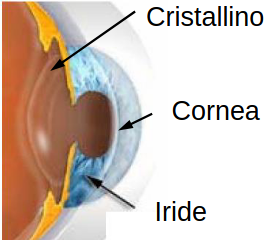
\includegraphics[width=0.4\linewidth]{chapters/images-chap7/struttura-iride.png}
\end{figure}

\section{Unicità dell'iride}

Come nel caso delle impronte, \textbf{non esistono due iridi uguali}.

Durante la formazione dell'iride si hanno delle componenti casuali che 
producono un pattern di righe, tagli e pieghe (le feature iridee) \textbf{unico
e distinguibile}.

Anche i gemelli omozigoti hanno iridi diverse.

\begin{figure}[ht]
    \centering
    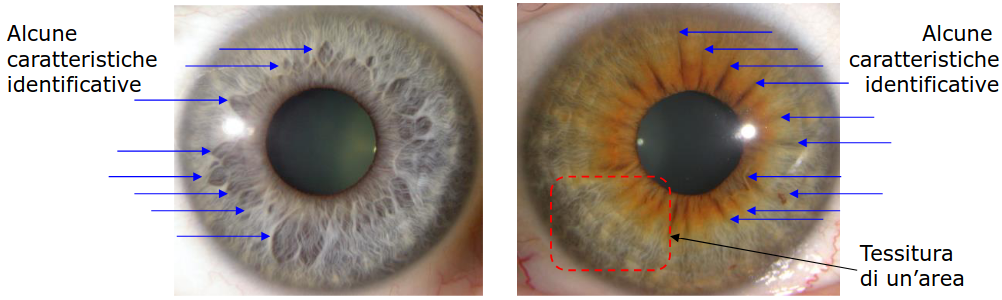
\includegraphics[width=1\linewidth]{chapters/images-chap7/unicita.png}
\end{figure}

Le feature più interessanti per il sistema biometrico si \textbf{vedono meglio con luce IR} 
piuttosto che la luce visibile.

È necessario inoltre usare \textbf{telecamere con ottiche variabili} per trovare
l'occhio nel volto e poi zoomare verso l'occhio per acquisirlo alla massima
risoluzione possibile.

\section{Rappresentazione delle iridi}
I moderni sistemi per il riconoscimento basati sull'iride rappresentano l'iride come 
una stringa di bit, chiamata \textbf{iriscode}.

I passi che permettono di passare da una immagine di un occhio ad un iriscode sono:
\begin{enumerate}
    \item individuazione dei centri e raggi della pupilla e dell'iride 
    \item rimozione della parte non utile occupata da ciglia 
    \item linearizzazione dell'iride
    \item trasformazione dell'iride linearizzata in wavelet
    \item trasformazione della trasformata wavelet in bit, ovvero iriscode
\end{enumerate}

\subsection{Calcolo dei centri e raggi di iride e pupilla}
Viene trovato l'occhio nell'immagine del volto, successivamente la pupilla 
e il raggio esterno dell'iride.

\subsection{Rimozione di palpebre e ciglia}
Solo una parte dell'iride è utile al riconoscimento; occorre segmentare 
solo la parte utile dell'iride.

Se manca più del 50\% dell'iride occorre riacquisire l'immagine.